\documentclass[spanish]{udpreport}
\usepackage[utf8]{inputenc}
\usepackage[spanish]{babel}
\usepackage{graphicx}
\usepackage{caption}
\usepackage{subcaption}

% Podemos establecer el logo de alguna entidad o dejar el de la UDP (defecto)
%\setlogo{EITFI}

\title{Informe:\\ STP y VLAN\\Laboratorio Nº4, Redes de Datos}
\author{Grupo 3\linebreak \linebreak Henry López del Pino\\ Rocío Venegas\\ Cristóbal Oyarce}
\email{henry.lopezdelpino@mail.udp.cl \\ rocio.venegas@mail.udp.cl \\ cristobal.oyarce@mail.udp.cl}
\professor{Profesor: Jaime Álvarez \\ Ayudante: Maximiliano Vega}
\date{19 de Mayo de 2016}

% Además podemos establecer la facultad y escuela
% los valores por defecto son los siguientes:
%\udpschool{Escuela de Informática y Telecomunicaciones}
%\udpfaculty{Facultad de Ingeniería}
%\udpuniversity{Universidad Diego Portales}

\begin{document}
\maketitle

\tableofcontents

\chapter{Introducción}

En esta experiencia se estudiará el protocolo STP, en el cual el principal objetivo es impedir la creación de bucles, los bucles en la red se generan porque se habilitan dos o mas caminos para llegar al mismo destino, lo que produce caminos redundantes y los paquetes se demoran mas en llegar a su destino, por tomar un camino no optimo, produciendo fallos o la caída de la red. 
\\

Por otro lado, también aprenderemos como configurar e implementar una VLAN. Las VLAN  son una forma donde los administradores de red crean dominios de difusión lógicos  puedan expandirse a través de switches,  sin importar la ubicación física. Esto resulta conveniente para disminuir el tamaño de los dominios de difusión o para poder administrar de manera lógica grupos son tener la misma ubicación física.  

\chapter{Configuración de STP y red VLAN}

\section{STP en una red}

Para las actividades 1, 2 y 3 se creo una red en cisco packet tracer como se mostrara a continuación. 

\subsection{Topología base con bucle}

La red creada consiste de tres switches conectados entre si, como se puede ver en la imagen:
\begin{figure}[htb]
\centering
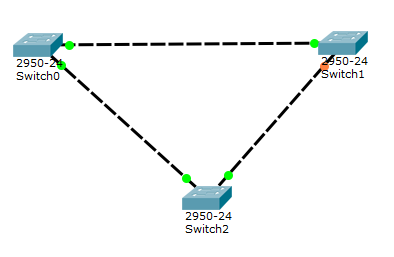
\includegraphics[width=5.5cm, height=3.5cm]{photos/red_original.png}
\caption{Red base con bucle} \label{fig:photos/red_original.png}
\end{figure}

\subsection{Configuración de STP}

A través de la interfaz de comandos de cisco packet tracer, se asignó el switch 1 como primario, y los switches 0 y 2 como secundarios.

\begin{figure}[htb]
    \centering
     \begin{subfigure}[b]{0.3\textwidth}
        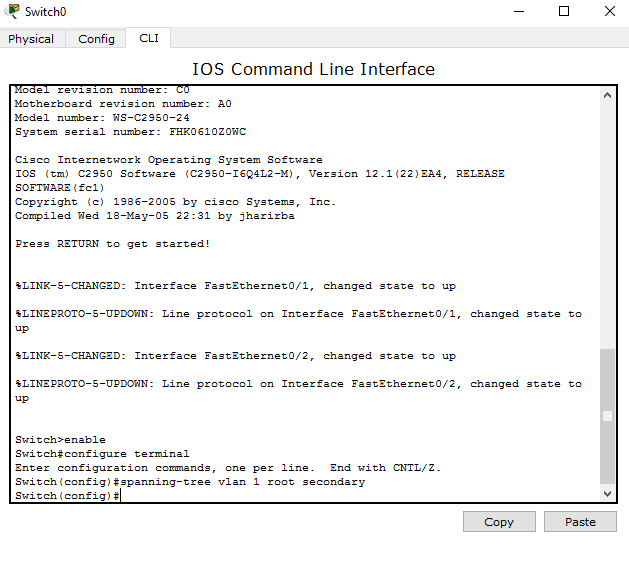
\includegraphics[width=\textwidth]{photos/switch_0_secundario.png}
        \caption{Switch 0} \label{fig:photos/switch_0_secundario.png}
    \end{subfigure}
    ~
    \begin{subfigure}[b]{0.3\textwidth}
        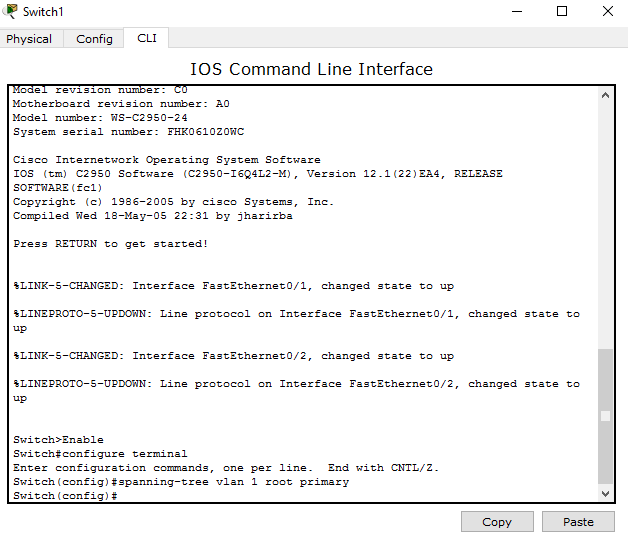
\includegraphics[width=\textwidth]{photos/switch_1_primario.png}
        \caption{Switch 1} \label{fig:photos/switch_1_primario.png}
    \end{subfigure}
    ~
    \begin{subfigure}[b]{0.3\textwidth}
        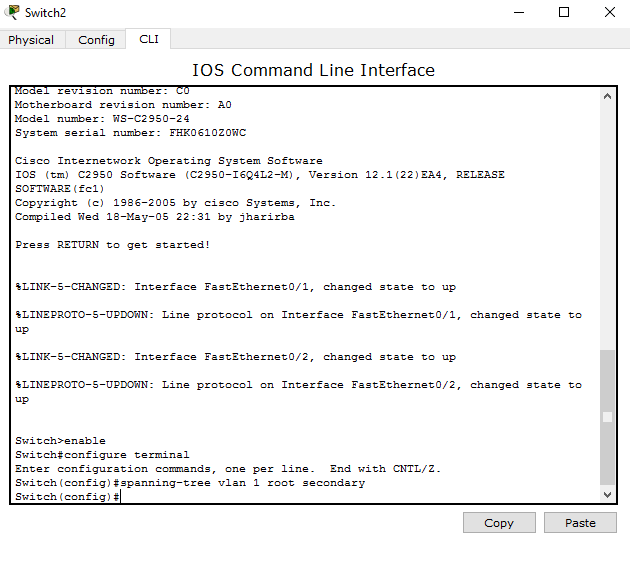
\includegraphics[width=\textwidth]{photos/switch_2_secundario.png}
        \caption{Switch 2} \label{fig:photos/switch_2_secundario.png}
    \end{subfigure}
    \caption{Configuración STP de los switches}
\end{figure}
\newpage
Luego de asignar la configuración STP a los switches, la red cambio la configuración de los puertos.

\begin{figure}[htb]
\centering
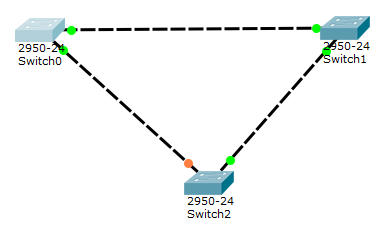
\includegraphics[width=5.5cm, height=3.5cm]{photos/red_despues_de_configurar_switchs.png}
\caption{Resultado de configuración STP} \label{fig:photos/red_despues_de_configurar_switchs.png}
\end{figure}

\subsection{Priorización en STP}

Otro metodo de configuración STP es el cambio de prioridad de cada switch, en el que se define que el que tenga menor prioridad es el mejor. Configurando el switch 2 con una prioridad 0, este quedo como primario.

\begin{figure}[htb]
    \centering
     \begin{subfigure}[b]{0.3\textwidth}
        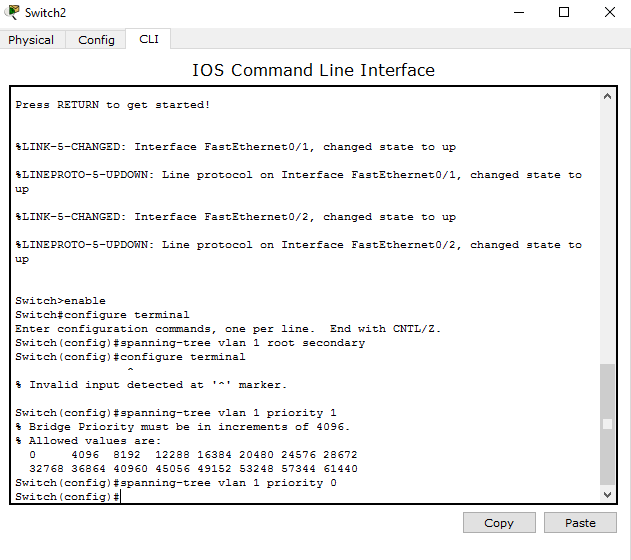
\includegraphics[width=\textwidth]{photos/switch_2_prioridad_0.png}
        \caption{Cambio prioridad} \label{fig:photos/switch_2_prioridad_0.png}
    \end{subfigure}
    ~
    \begin{subfigure}[b]{0.3\textwidth}
        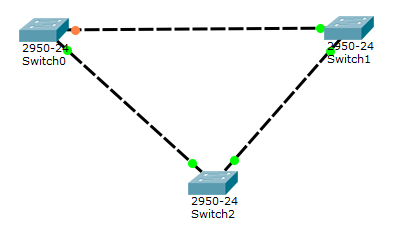
\includegraphics[width=\textwidth]{photos/resultado_cambio_prioridad.png}
        \caption{Resultado de cambio de prioridad} \label{fig:photos/resultado_cambio_prioridad.png}
    \end{subfigure}
    	\caption{Cambio de prioridad en switch 2}
\end{figure}

Realizando un segundo cambio a la prioridad, se asigno al switch 0 la prioridad 4096. En este caso el switch 2 se mantuvo como primario, pero hubo un cambio en los puertos bloqueados.

\begin{figure}[htb]
    \centering
     \begin{subfigure}[b]{0.3\textwidth}
        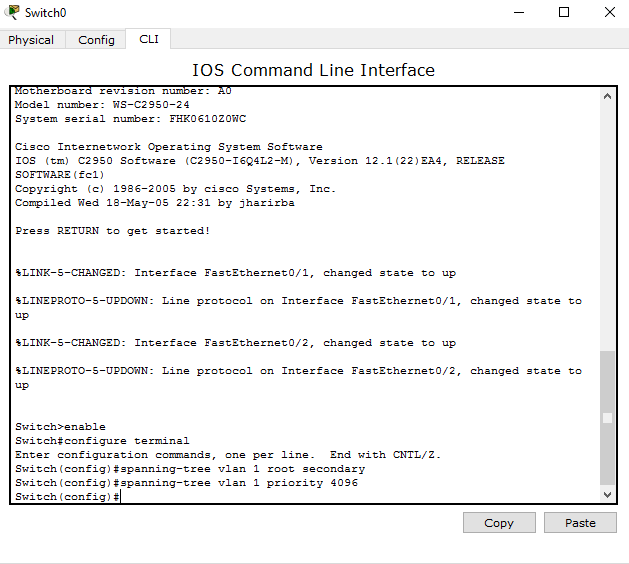
\includegraphics[width=\textwidth]{photos/switch_0_prioridad_4096.png}
        \caption{Cambio prioridad} \label{fig:photos/switch_0_prioridad_4096.png}
    \end{subfigure}
    ~
    \begin{subfigure}[b]{0.3\textwidth}
        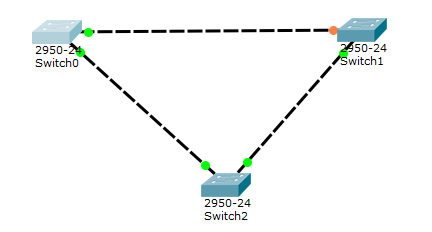
\includegraphics[width=\textwidth]{photos/resultado_cambio_prioridad_2.png}
        \caption{Resultado de cambio de prioridad} \label{fig:photos/resultado_cambio_prioridad_2.png}
    \end{subfigure}
    	\caption{Cambio de prioridad en switch 0}
\end{figure}

\section{Red VLAN}

Una  VLAN permite que un administrador de red cree grupos de dispositivos conectados a la red de manera lógica que actúan como si estuvieran en su propia red independiente, incluso si comparten una infraestructura común con otras VLAN.
\\
Se creará una red compuesta por varios switches y PCs, la cual posteriormente se le configuraran distintas VLAN.

\begin{figure}[htb]
\centering
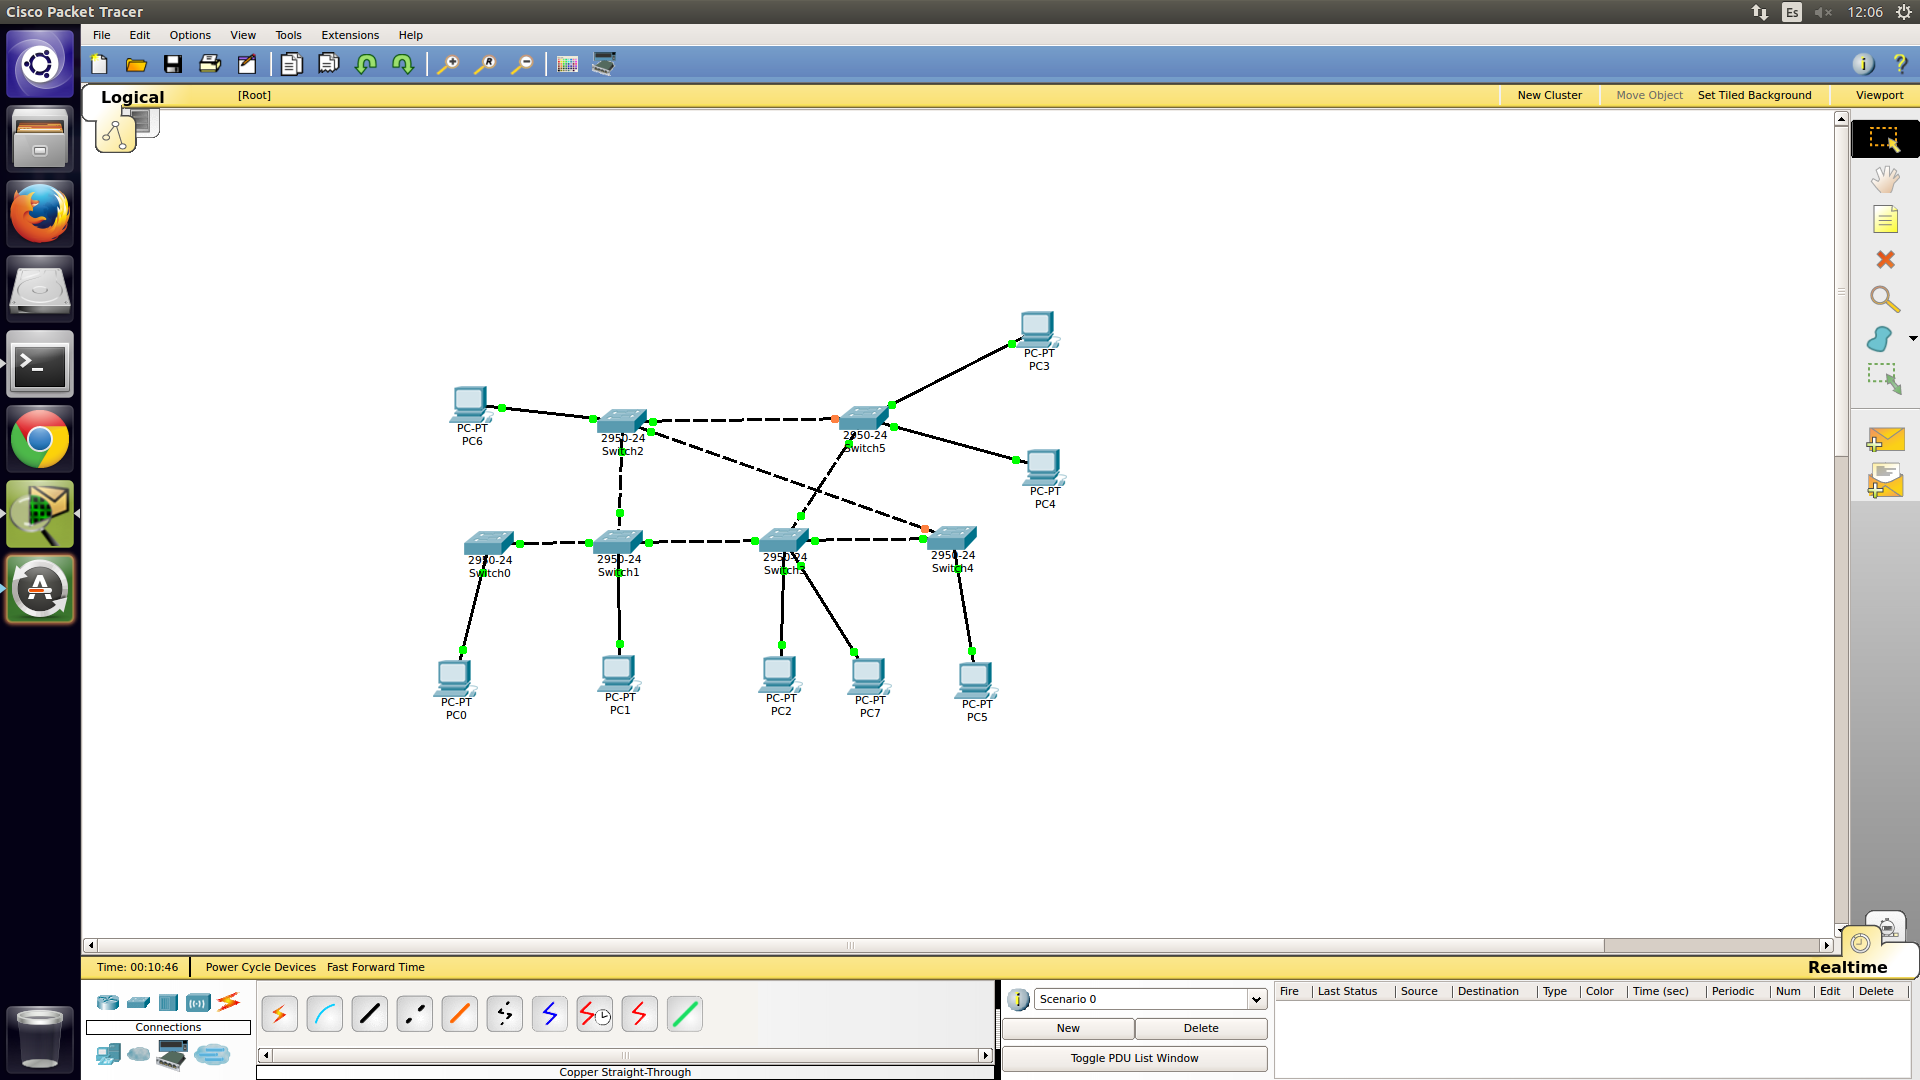
\includegraphics[width=5.5cm, height=3.5cm]{photos/VLAN_red.png}
\caption{Red VLAN} \label{fig:photos/VLAN_red.png}
\end{figure}



\subsection{Configuración VLAN}

A la red creada se le asignó distintas VLAN a los switches y PCs, se configuraron puertos como puertos trunk y otros como puertos access, como se podrá ver en la imagen siguiente:

\begin{figure}[htb]
\centering
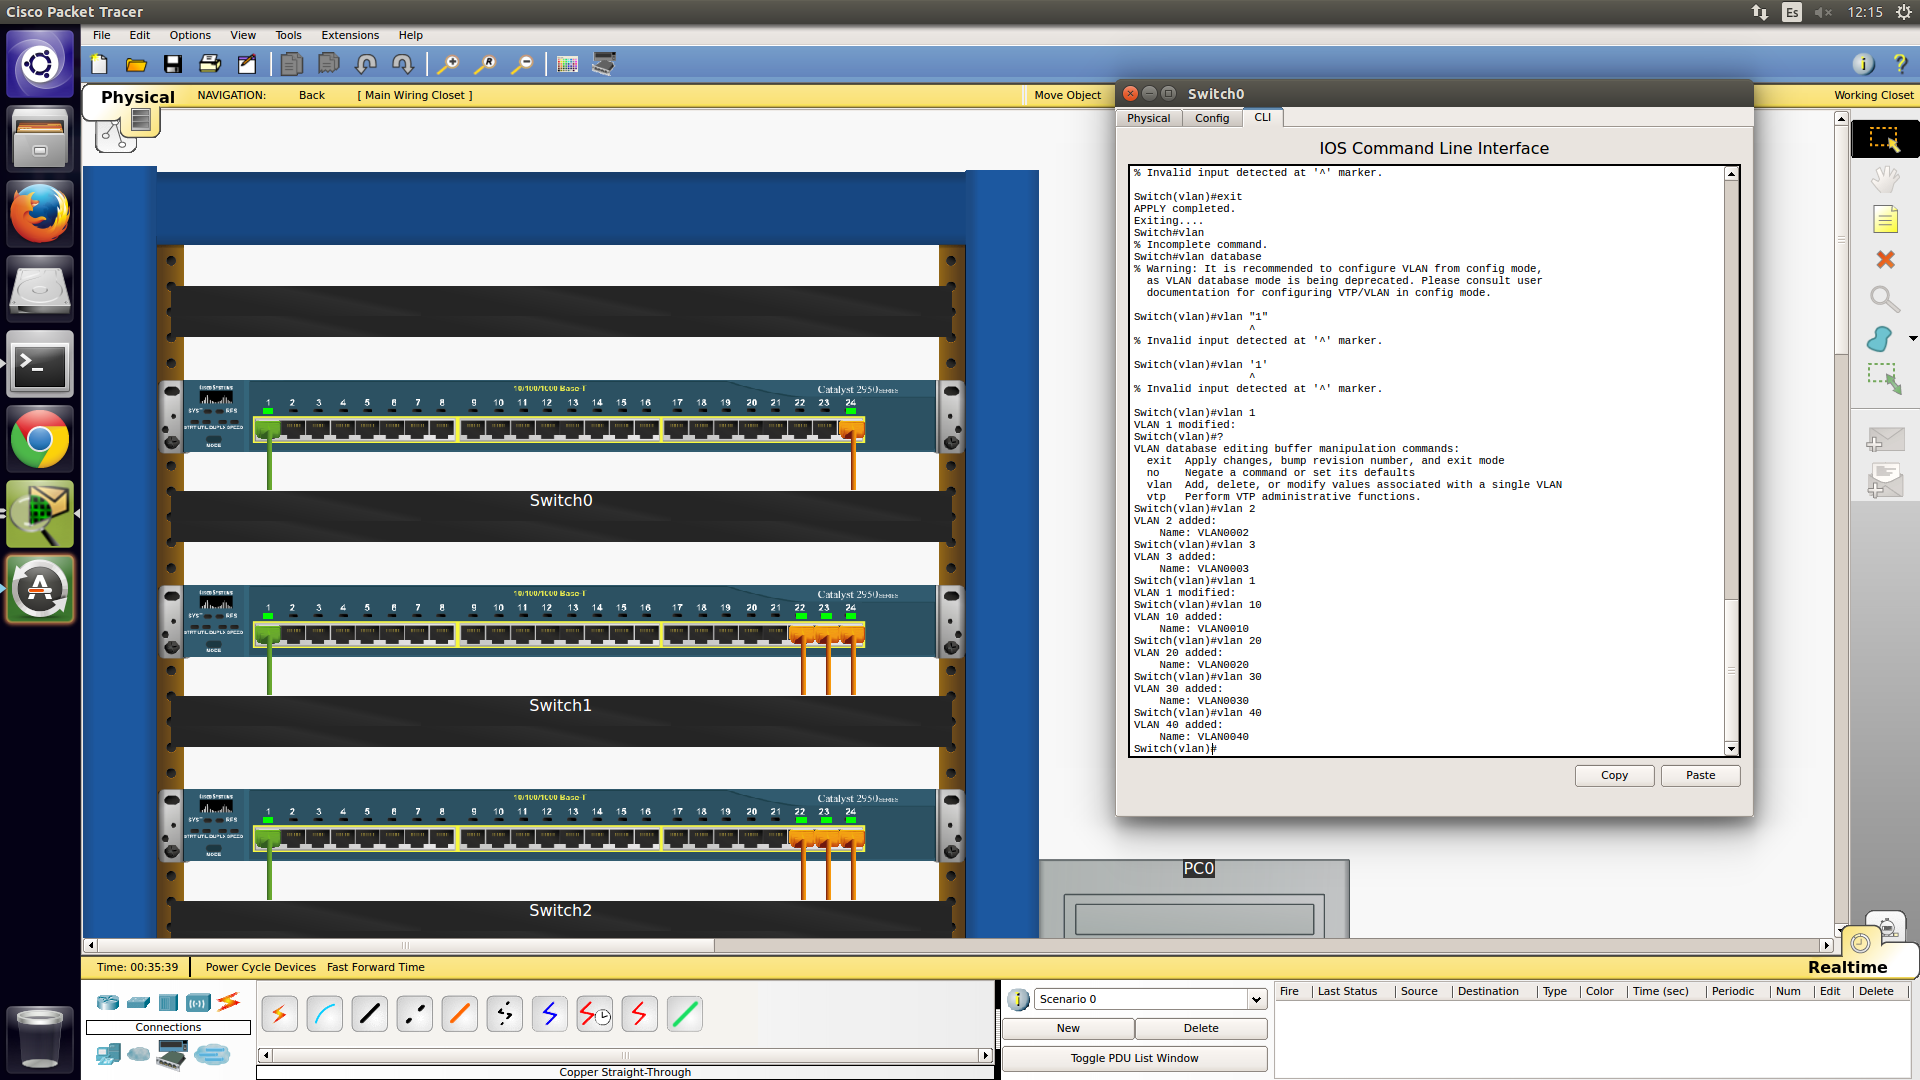
\includegraphics[width=5.5cm, height=3.5cm]{photos/VLAN_rack.png}
\caption{Configuración VLAN en los switches} \label{fig:photos/VLAN_rack.png}
\end{figure}

Luego de esto se realizó distintas pruebas de ping entre equipos pertenecientes a la VLAN y equipos de distintas VLAN.

\chapter{Conclusiones}
\section{Conclusiones Generales}


En la red, si el switch primario no se asigna de forma manual, los switches asignarán uno, también se puede asignar el switch primario a través de comandos o asignando prioridades a cada switch, el switch con menor prioridad quedará como el switch primario. De esta forma la red no tendrá bucles en el envió de paquetes debido a que se bloquearan puertos en los switches secundarios.
\\



\newpage
\section{Respuesta a cuestionarios propuestos}
\subsection{Cuestionario (ACTIVIDAD I Y ACTIVIDAD II)}
\subsubsection {¿Qué camino realizara un paquete que para llegar desde el switch
0 hasta el switch2? (ACTIVIDAD I)}
El camino que realizó el paquete para llegar del switch 0 al swicth 2, fue directo a través de los switches.
\subsubsection{¿Qué camino realizara un paquete que para llegar desde el switch
2 hasta el switch1? (ACTIVIDAD I)}
El camino que realizó el paquete para llegar del switch 2 al swicth 1, fue  a través del switch 0.

\subsubsection{ ¿Qué camino realizara un paquete que para llegar desde el switch
2 hasta el switch0? (ACTIVIDAD II)}
El camino que realizó el paquete para llegar del switch 2 al swicth 0, fue  a través del switch 1.
\subsubsection{ ¿Qué camino realizara un paquete que para llegar desde el switch 1 hasta el switch0? (ACTIVIDAD II)}
El camino que realizó el paquete para llegar del switch 0 al swicth 2, fue directo a través de los switches.
\newpage
\subsection{Cuestionario (ACTIVIDAD IV)}
\subsubsection {¿Cuál es la diferencia del modo Access y el modo Trunk en un switch?}
el  modo conecta a solo una VLAN, a diferencia de modo trunk el cual permite conectar varias VLAN.
\subsubsection{¿Qué ocurre si conecto una puerta en modo Trunk a un PC?}

El PC va estar conectado a varias VLAN
\subsubsection{¿Qué ocurre si conecto dos switches, uno en modo access y otro en modo trunk?}
Los dos switches funcionaran como si estuvieran en modo access , porque los paquetes de trunk son descartados.
\subsubsection{¿Qué camino realizara un paquete que para llegar desde el switch 1 hasta el
switch 0?}
El camino que realizó el paquete para llegar del switch 1 al swicth 0, es directo a través de los switches.
\listoffigures

\end{document}